\documentclass[xetex,aspectratio=169]{beamer}
\usepackage{fontspec}
\usepackage{xltxtra}
\usepackage{xunicode}
\usepackage{pgfpages}
\usepackage{url}
\usepackage{takahashi}
\usepackage{listings}
\newcommand{\stack}[1]{\begin{tabular}{@{}c@{}}#1\end{tabular}}
\definecolor{mauve}{rgb}{0.58,0,0.82}
\definecolor{dkgreen}{rgb}{0.2,0.9,0.2}
\lstset{%
  language=Java,
  basicstyle=\scriptsize\fontspec{Input},
  breaklines=true,
  showspaces=false,
  showstringspaces=false,
  keywordstyle=\color{blue},
  commentstyle=\color{dkgreen}\itshape,
  stringstyle=\color{mauve},
  numberstyle=\color{red!75}
}

% make pgfpages and xelatex play nicely together.
% I don't know why this works, the Internet told me to do it.
\renewcommand\pgfsetupphysicalpagesizes{%
    \pdfpagewidth\pgfphysicalwidth\pdfpageheight\pgfphysicalheight%
}

\usefonttheme{professionalfonts}
\setsansfont[BoldFont=Whitney SSm Semibold,Mapping=tex-text]{Whitney SSm Book}
\setmonofont{Input}
%\setdefaultlanguage{english}
\usecolortheme{crane}
\setbeamertemplate{navigation symbols}{}
\setbeamertemplate{caption}[numbered]
\setbeameroption{show notes on second screen=right}

\title[Localization]{How We Approach Localization at Meetup}
\author{Mike Castleman}
\institute[Meetup]{Meetup, Inc.}
\date[2015-03-19]{March 19, 2015}
\begin{document}

\begin{frame}
\titlepage
\end{frame}

\takahashi{\stack{A Brief\\Apology}}
\note{Ich kann nur Englisch sprechen.}

\takahashi{
\includegraphics{meetuplogo.pdf}}
\note{so, like, what's ``Meetup''? maybe you have some idea?}

\takahashi{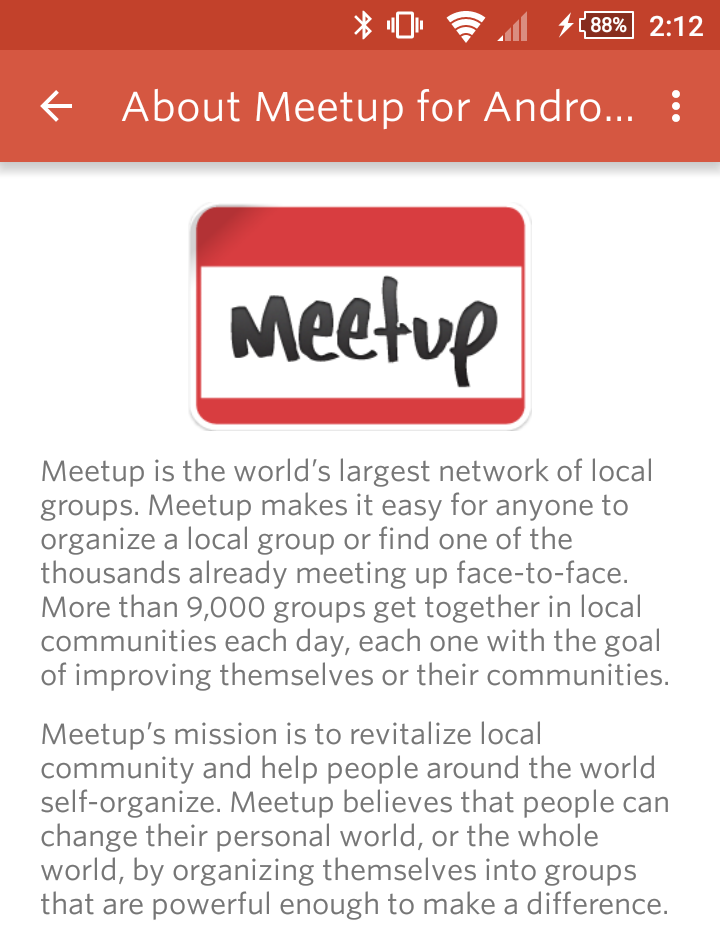
\includegraphics{about-meetup.png}}
\note{I'm lazy and didn't want to write any copy… this copy is old and the numbers are wrong but whatever}

\takahashi{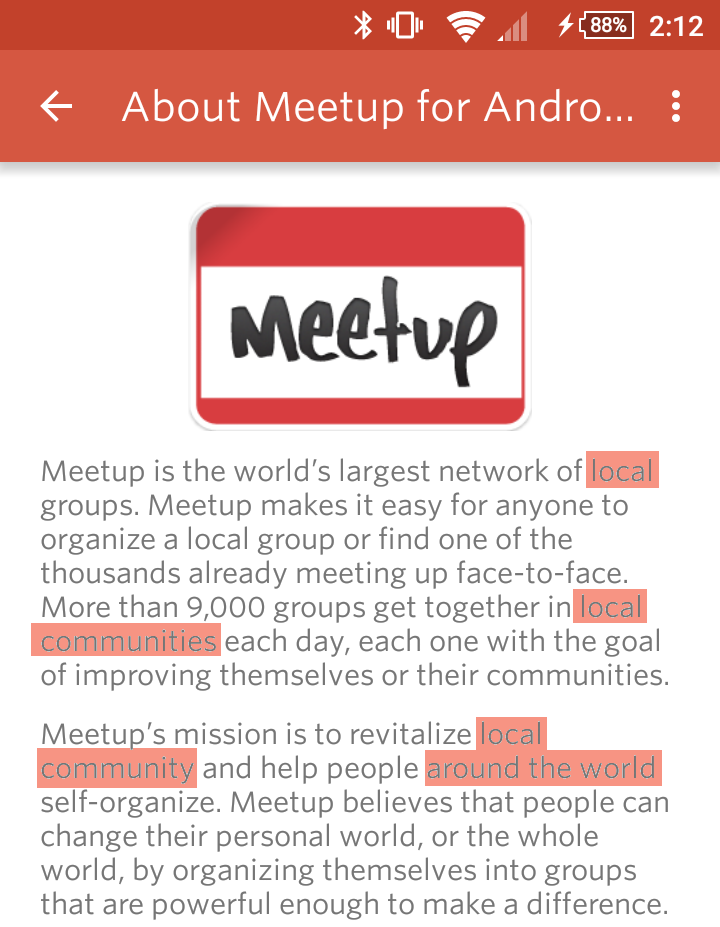
\includegraphics{about-meetup-hl.png}}
\note{HM. A theme…? But HOW CAN WE DO IT?}

\takahashi{A Problem}

\takahashi{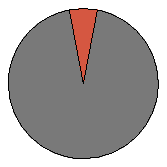
\includegraphics{piechart.pdf}}
\note{ca.~6\% of the world is a native speaker of English}

\takahashi{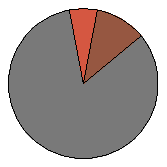
\includegraphics{piechart-2.pdf}}
\note{an additional 11\% can speak English as a second or third language}

\takahashi{l10n}
\note{localization yo! We'll talk primarily about how to do the technical part here, but obvs you need to be sensitive to other local needs etc etc yeah}

\takahashi{\stack{Which\\lanugages?}}

\takahashi{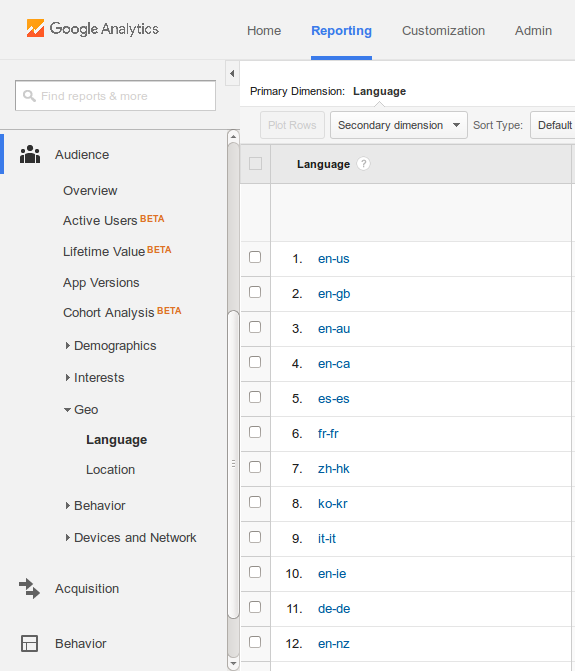
\includegraphics{analytics.png}}
\note{do your market research… every business is different. if you're looking at GA, maybe like sum \texttt{en-us} and \texttt{en-ca}.}

\takahashi{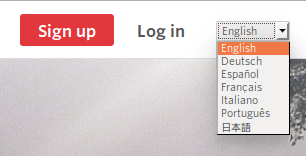
\includegraphics{desktop-lang-picker.png}}
\note{like, supporting all the same languages as on dweb is not a \textit{terrible} choice. japanese launched recently; korean coming soon(ish).}

% TK TK Graph of upwards slope in ja reg or something.

\takahashi{HOWTO}

\begin{frame}[<+->]{Process Overview}
\note{this is like the only bulleted list you'll see in this presentation.}
\begin{enumerate}
\item Write everything in English.
\item Translate it to other languages.
\item Profit!
\end{enumerate}
\end{frame}

\takahashi{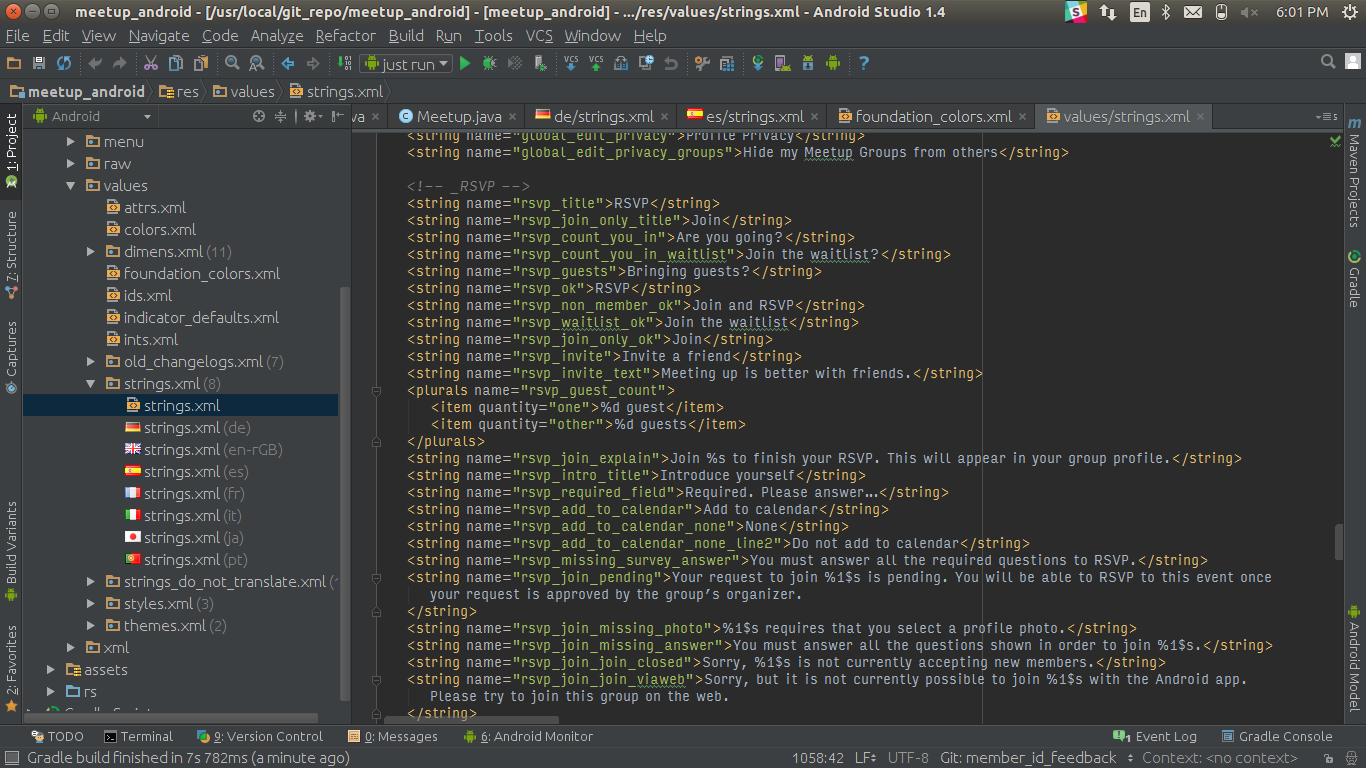
\includegraphics{strings-xml.png}}
\note{\begin{itemize}
\item translate all the strings.
\item fortunately, it's pretty easy on Android. like, I looked at Phil's slides on iOS localizations and it's maybe a three-step process with at-signs or something? not for us.
\item put all the strings to be translated in \texttt{strings.xml}.
\item like, actually, \textbf{all} of them. (much easier to get it right the 1st time than fix it later)
\item don't put all the strings not to be translated there.
\end{itemize}}

\takahashi{\texttt{<plurals/>}}
\note{super-useful!}

\takahashi{\stack{\onslide<1->{0 days, 1 day, 2 days}\\
\onslide<2->{0 días, 1 día, 2 días\\0 Tage, 1 Tag, 2 Tage}\\
\onslide<3->{0 \textbf<3>{jour}, 1 jour, 2 jours}\\
\onslide<4->{\fontspec{TakaoMincho}{0日、1日、2日}}\\
\onslide<5>{za 0 mjeseci, za 1 mjesec, za 2 mjeseca}}%
\note<1>{english} \note<2>{spanish, german} \note<3>{french} \note<4>{japanese} \note<5>{croatian\par Fortunately, Android offers to take care of all of this for you! Let it.}}

\takahashi{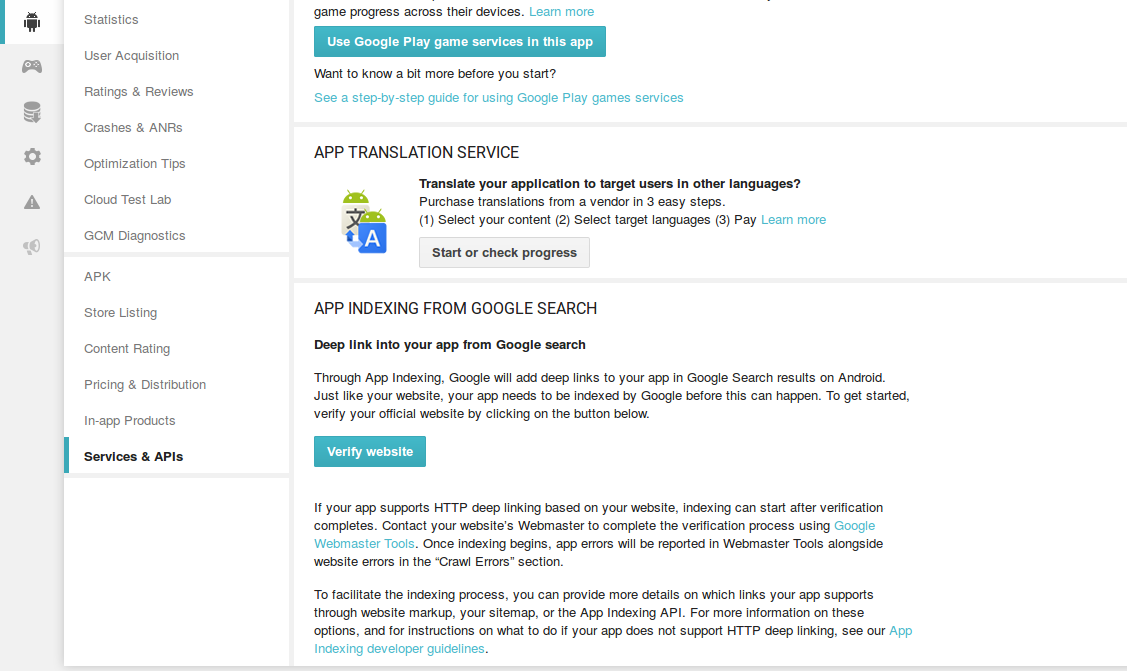
\includegraphics{app-translation-svc-1.png}}
\note{our first try at translating the android app. it's easy enough to use and works sort of okay, but…}

\takahashi{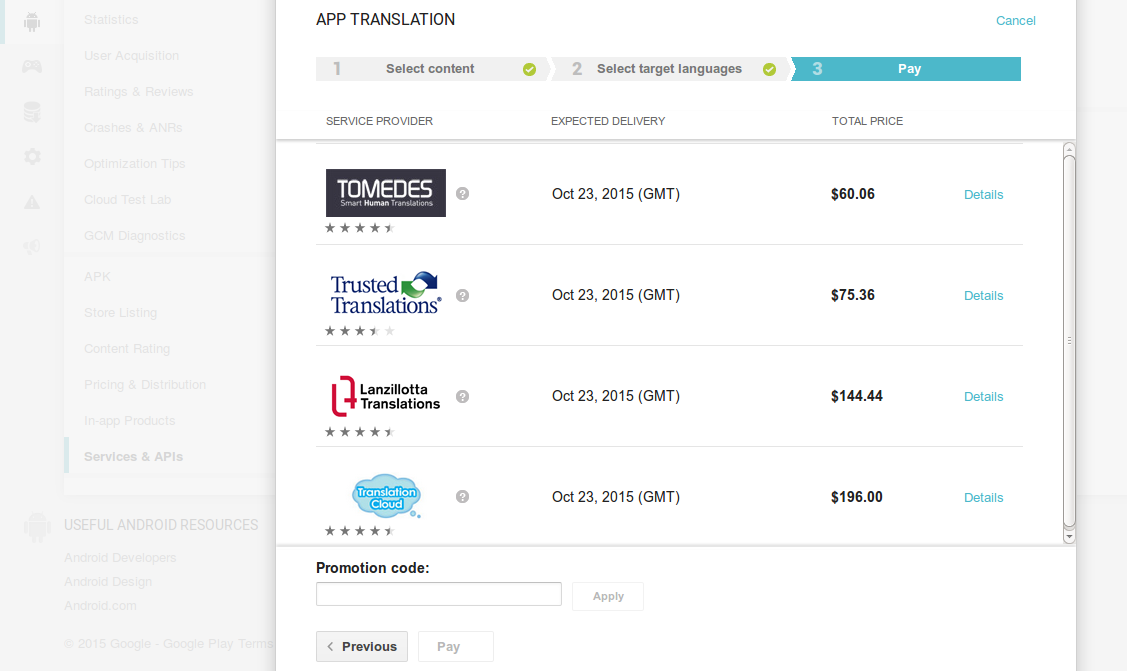
\includegraphics{app-translation-svc-2.png}}
\note{you're just dumped in this weird world where you have to pick amongst all these providers, and no one cares about anything except price}

\takahashi{\stack{\onslide<1->{Use }\onslide<2->{human}\\\onslide<3>{native-speaker}\\\onslide<1->{translators.}}%
\note<2>{it's really hard to expect to rely on crowdsourcing for languages your app isn't yet popular in. maybe twitter can get away with it, but you probably can't. and contract translators may be okay but won't know and love your product, nor can they be expected to use consistent terminology.}%
\note<3>{so like obviously whatever you can do is what you should do. can you open an office in every country in which you do business? can you buy your friend a beer to fix the most egregious errors in third-party translations?}}

\takahashi{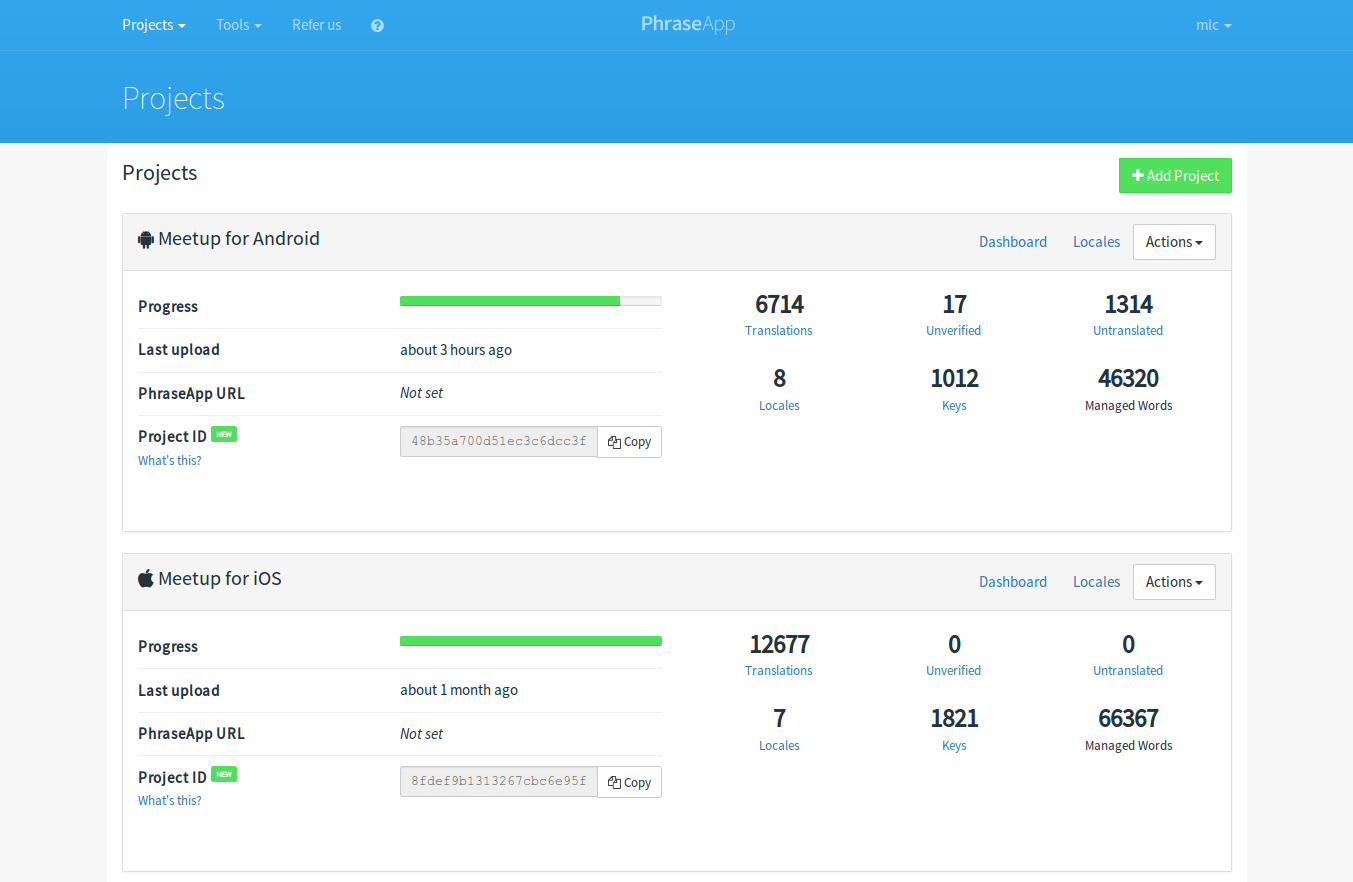
\includegraphics{phraseapp.png}}
\note{so, we use this thing called phraseapp for managing our translations. it's pretty good, and not free but cheaper than many of the (worse) alternatives. very startuppy, \&c.}

\takahashi{\input{phraseapp-workflow.pdf_tex}}
\note{workflow. don't modify English inside translation tool, nor other languages outside of it}

\takahashi{Layout}

\takahashi{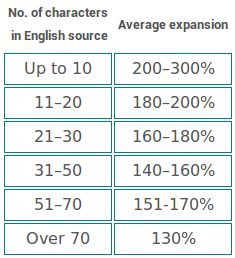
\includegraphics{w3c-text-lengths.png}}
\note{source: IBM \textit{Guidelines to design global solutions}, via W3C's \textit{Text size in translation} \url{http://www.w3.org/International/articles/article-text-size.en}}

\takahashi{\stack{\onslide<1->{Use the tools}\\\onslide<2>{you already know.}}%
\note<2>{your layouts already have to deal with:
\begin{itemize}
\item varying device sizes
\item varying user-set text sizes
\end{itemize}
l10n is just another piece of the puzzle.}}

\takahashi{\stack{\onslide<1->{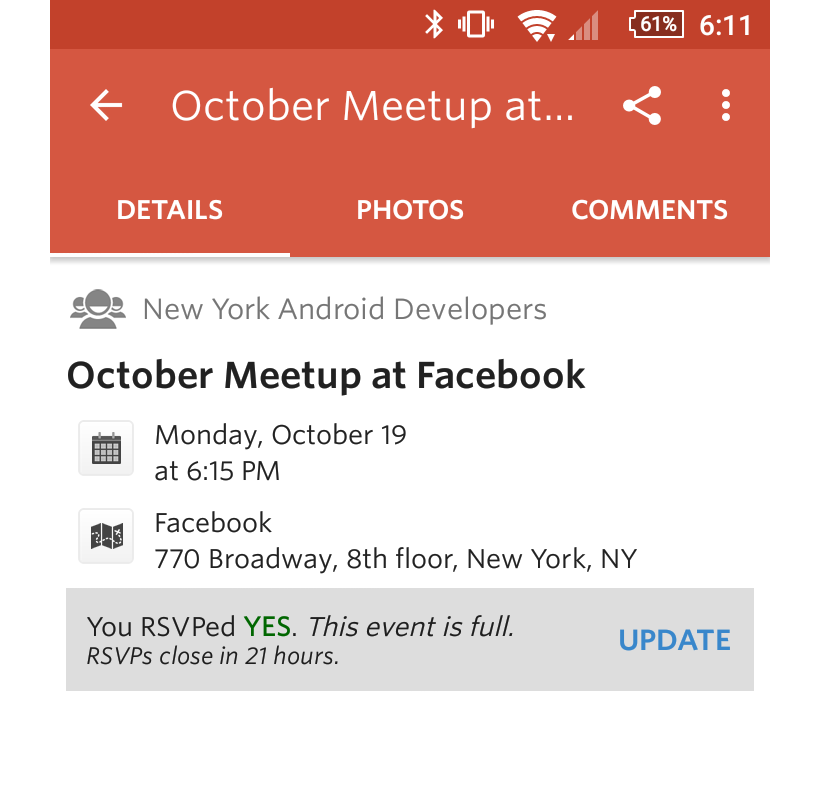
\includegraphics{rsvp1.png}}\\\onslide<2>{\fontsize{24}{30}{\texttt{android:layout\_weight="1"\ \ \ \ \ \ android:layout\_width="wrap\_content"}}}}}

\takahashi{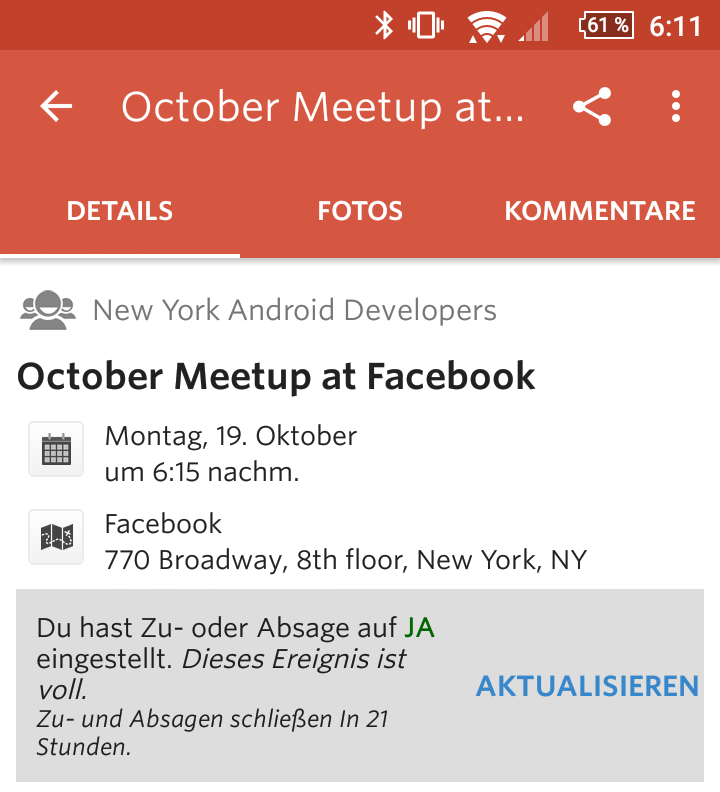
\includegraphics{rsvp2.png}}
\note{So far, so good. You'll notice also that we

\textbf{protip!} Memorize where the change-language setting is on your device, so you can get back to English!}

\takahashi{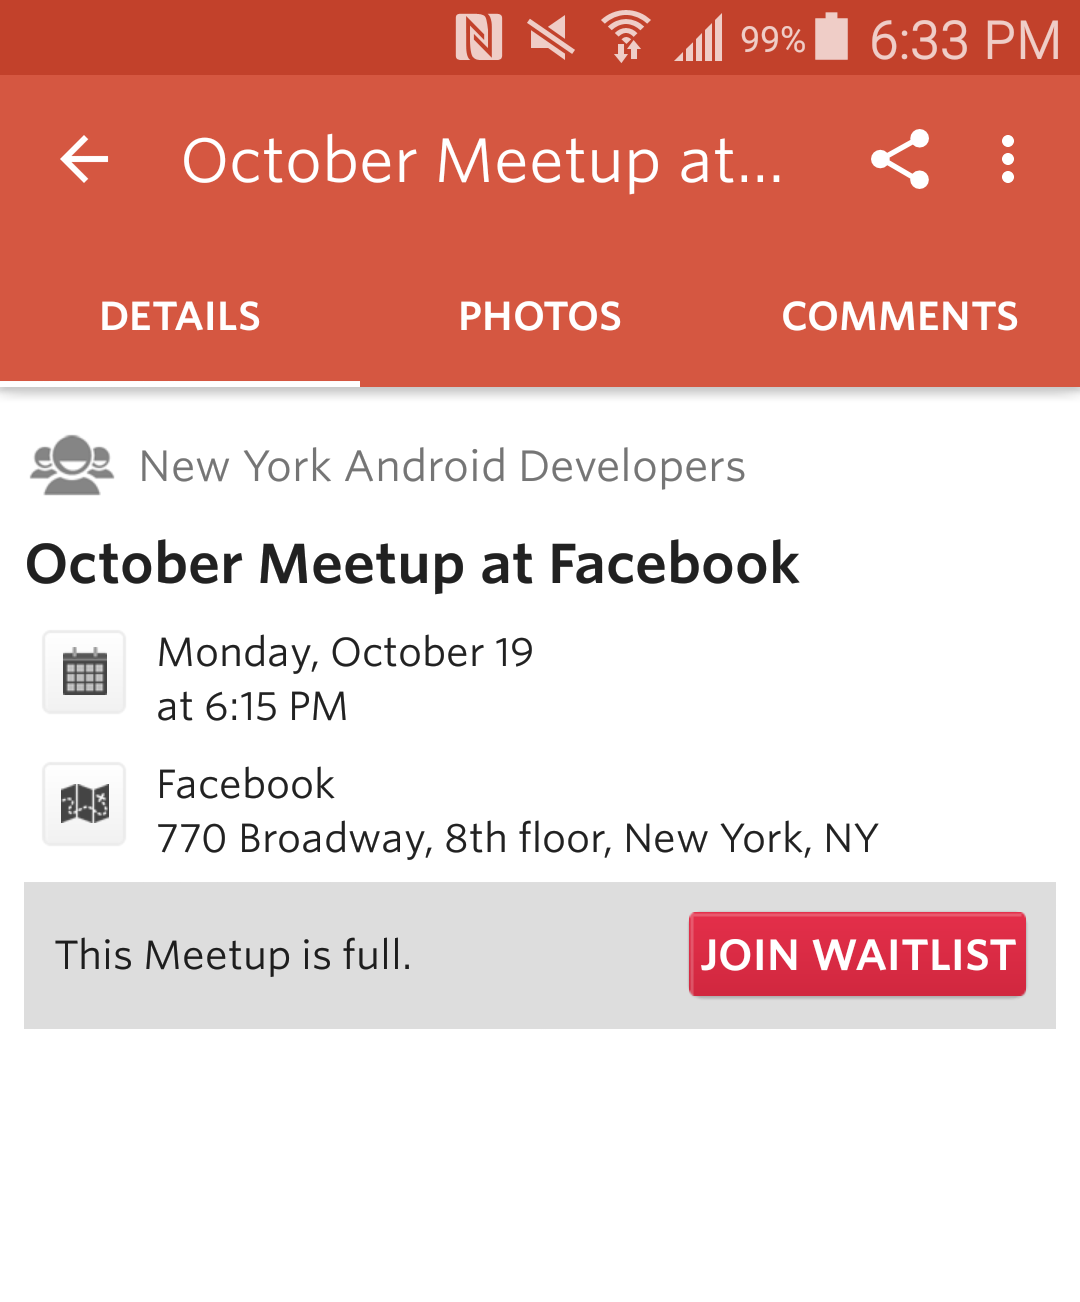
\includegraphics{rsvp3.png}}
\note{wow Android is rly good…}

\takahashi{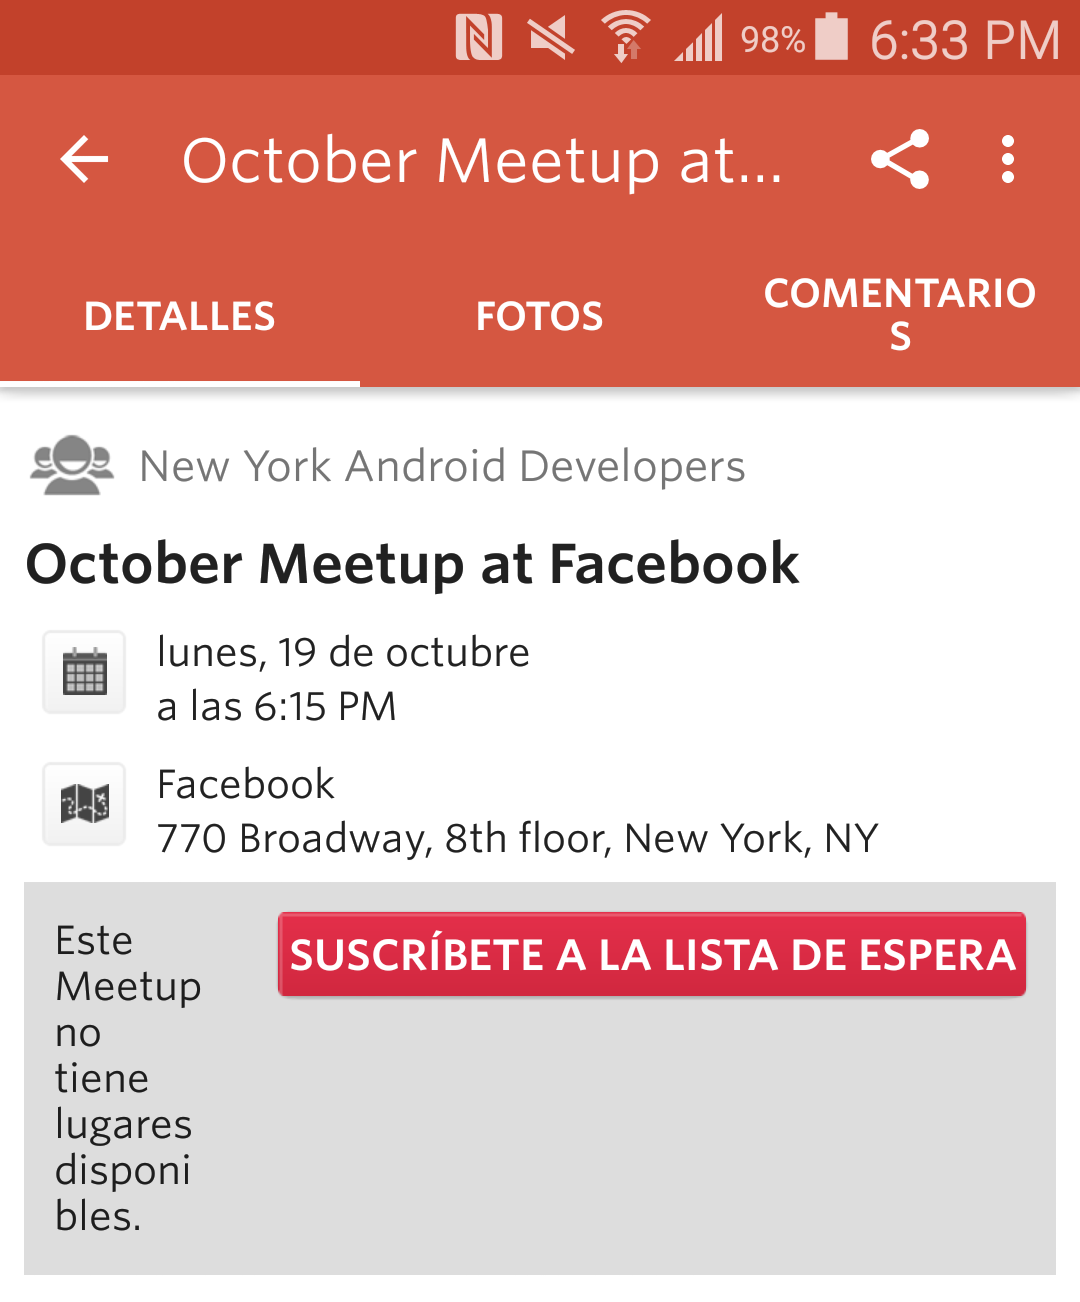
\includegraphics{rsvp4.png}}
\note{…but not magic. rejigger your layout, or use the humans you have who know and love your product to figure out a shorter way to say what you want.}

\begin{frame}[fragile]
\note{sometimes you can fit longer copy on most devices but not all; we use this especially for buttons at the bottom of the screen.}
\begin{lstlisting}
/**
 * Attempts to set copy into a TextView using the normal copy. If it ends up
 * wrapping onto more than one line, uses the short copy alternative instead.
 * @param textView The TextView (or Button or whatever) to setText on.
 * @param normalCopyResId The preferred copy string resource id.
 * @param shortCopyResId The alternate (shorter) copy string resource id.
 */
public static void maybeUseShorterCopy(final TextView textView,
                                       @StringRes final int normalCopyResId,
                                       @StringRes final int shortCopyResId) {
    textView.post(() -> {
        // posting to the view ensures that it's been laid out and sized first
        textView.setText(normalCopyResId);
        if (textView.getLineCount() > 1) {
            textView.setText(shortCopyResId);
        }
    });
}
\end{lstlisting}
\end{frame}

\takahashi{Dates \& Times}

\takahashi{\stack{
\onslide<1->{Monday, October 19}\\
\onslide<2->{Monday, 19 October}\\
\onslide<3->{Montag, 19. Oktober}\\
\onslide<4->{lunes, 19 de octubre}}}

\takahashi{\stack{If you try to do\\
this yourself, \onslide<2>{there\\
\textbf{will} be bugs.}}}

\takahashi{CLDR}
\note{\begin{itemize}
\item ``Common Locale Data Repository''
\item part of Unicode
\item basis for Android l10n stuff
\item but sometimes it's useful to look at their website and take things from there
\end{itemize}}

\takahashi{\stack{\texttt{DateUtils.formatDateTime}\\
\texttt{DateUtils.formatDateRange}\\
\texttt{DateUtils.formatElapsedTime}}}
\note{There's lots of garbage in the Android SDK, but these methods are srsly battle-tested. Even then, we've found (subtle) bugs in pre-KitKat implementations! Maybe you want to read the source?}

\takahashi{\texttt{libcore.icu.ICU}}
\note{hidden, private internal API. but maybe for some things you want to call it by reflection anyway. you'll need a fallback though for platforms where it's unavailable. some useful stuff like words for ``yesterday'' and ``today'', and slightly lower-level date formatting.}

\takahashi{Sorting}

\takahashi{\texttt{String implements Comparable<String>}}

\takahashi{\stack{Apple\\Orange\\banana}}

\takahashi{\texttt{String.CASE\_INSENSITIVE\_ORDER}}
\note{works okay for English, but not for all languages. like German ß or what have you}

\takahashi{\texttt{java.text.Collator}}
\note{getting there!}

\takahashi{TK TK: screenshot of Japanese onboarding screen}
\note{but sometimes, sorting \textit{can not be done by a computer}. \url{http://www.localizingjapan.com/blog/2011/02/13/sorting-in-japanese-\%E2\%80\%94-an-unsolved-problem/} Again, this is something that a human who cares about your product may tell you, but a 5¢/word translation service will not.}

\begin{frame}{Stay in touch!}
\note<1>{omg another bullet list}
\Large{\onslide<1->{\begin{itemize}
\item mike castleman
\item \texttt{mlc@meetup.com}
\item \texttt{@vermicelli}
\end{itemize}}
\vskip 5ex
\onslide<2>{We're hiring!}}
\end{frame}

\end{document}
